%TeX

\section{Finding the flag}

\begin{frame}{A quick recap\ldots}
    \begin{columns}
        \column{0.5\textwidth}
        \begin{itemize}
            \item<1-> We have an x86 boot sector that's asking us for the flag
            \item<2-> The flag is clearly in the boot sector SOMEWHERE\ldots
            \begin{itemize}
                \item<3-> \ldots but not in plaintext, because this is a 400
                          point challenge and that would be too easy
            \end{itemize}
            \item<4-> So, where is it?
        \end{itemize}
        \column{0.5\textwidth}
        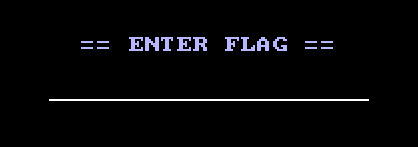
\includegraphics[width=\textwidth]{enter-flag}
    \end{columns}
\end{frame}

\begin{frame}{Reversing the boot sector}
    \begin{columns}
        \column{0.5\textwidth}
        \begin{itemize}
            \item<1-> Open the file in your favorite disassembler (e.g. IDA);
                      rebase at \texttt{0x7c00}
            \item<2-> We can visally pick out three sections:
            \begin{itemize}
                \item<2-> Init code (responsible for the protected
                          mode transition)
                \item<2-> Display code (identifiable by a large number of
                          \texttt{int} instructions)
                \item<2-> Some other code that uses Intel SSE2 instructions
            \end{itemize}
        \end{itemize}
        \column{0.5\textwidth}
        \begin{tikzpicture}
            \only<1> {\node (cfg) {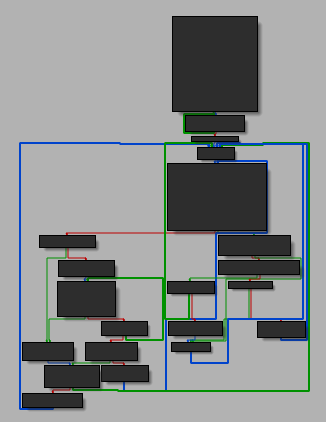
\includegraphics[width=\textwidth]{cfg}};}
            \uncover<2-> {\node (cfga) 
                {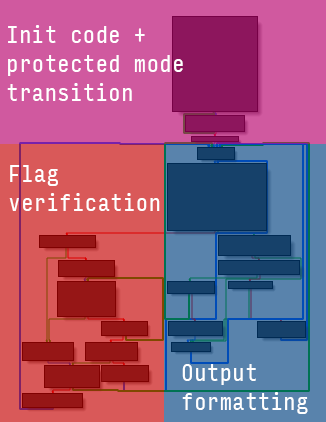
\includegraphics[width=\textwidth]{cfg-annotated}};}
        \end{tikzpicture}
    \end{columns}
\end{frame}

\begin{frame}{First leads}
    \begin{itemize}
        \item<1-> The program asks you to enter 20 characters, and immediately
                  breaks out if the first 4 characters aren't 'flag' after you
                  enter character \#20
        \item<2-> We can verify this in a debugger after eyeballing the code

        \begin{center}
            \uncover<3-> {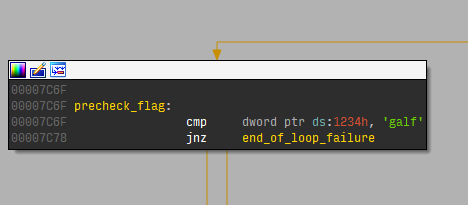
\includegraphics[width=0.7\textwidth]{flag-precheck}}
        \end{center}
    \end{itemize}
\end{frame}

\begin{frame}{As it turns out\ldots}
    \framesubtitle{After several hours of staring at x86 assembly}

    \begin{itemize}
        \item<1-> The flag is \alert{hashed} using a \alert{custom algorithm}
                  implemented with Intel SSE instructions
        \item<2-> {\em Ugh\ldots}
        \item<3-> We have to find an input to the hash algorithm that hashes
                  to the same value stored in the boot sector
    \end{itemize}
\end{frame}

\begin{frame}{Suddenly, SSE2 instructions}
    \framesubtitle{``My Intel CPU can do {\em that?}''}
    The author of the challenge decided to use a bunch of obscure x86 SSE2
    instructions to force us to trawl through Intel documentation

    \begin{itemize}
        \item<2-> movaps\uncover<3->{: Moves to/from/between XMM registers}
        \item<2-> \alert<4->{andps}\uncover<3->{: Performs bitwise AND between
                                                XMM registers}
        \item<2-> pshufd\uncover<3->{: Reorders 32-bit words in XMM registers}
        \item<2-> \alert<4->{psadbw}\uncover<3->{: Sums absolute values of
                                                 differences between bytes
                                                 (it's as crazy as it sounds)}
    \end{itemize}

    \begin{block}<1->{Note}
        SSE2 instructions operate on XMM registers, which are 128 bits
        (16 bytes) wide.
    \end{block}

    \begin{alertblock}<4>{Question}
        Why are these instructions useful for writing a hash function (even if
        it's a bad hash function that we can break?)
    \end{alertblock}
\end{frame}

\newcommand{\StartCell}[2]{
    \node at (0,0) (#1) {\texttt{#2}};%
}
\newcommand{\Cell}[3]{
    \node [anchor=west] at (#1.east) (#2) {\texttt{#3}};%
}

\newcommand{\Xmm}[2]{%
    \getargsC{#2}%
    \raisebox{0.5em}{\texttt{xmm#1}:\xspace}%
    \begin{tikzpicture}[%
        every node/.style={%
            minimum width=1.5em,
            minimum height=0.75em,
            text height=0.75em,
            text depth=0.25em,
            outer sep=0pt,
            draw=black,
            semithick
        }
    ]%
        \StartCell{A}{\argi}%
        \Cell{A}{B}{\argii}%
        \Cell{B}{C}{\argiii}%
        \Cell{C}{D}{\argiv}%
        \Cell{D}{E}{\argv}%
        \Cell{E}{F}{\argvi}%
        \Cell{F}{G}{\argvii}%
        \Cell{G}{H}{\argviii}%
        \Cell{H}{I}{\argix}%
        \Cell{I}{J}{\argx}%
        \Cell{J}{K}{\argxi}%
        \Cell{K}{L}{\argxii}%
        \Cell{L}{M}{\argxiii}%
        \Cell{M}{N}{\argxiv}%
        \Cell{N}{O}{\argxv}%
        \Cell{O}{P}{\argxvi}%
    \end{tikzpicture}%
}

\newcommand{\Left}[1]{\textcolor<5->{red}{#1}}

\newcommand{\Right}[1]{\textcolor<5->{orange}{#1}}

\begin{frame}{Packed Sum of Absolute Differences of Bytes in Word}
    \framesubtitle{That's a mouthful\ldots}
    \begin{center}
        \Xmm{0}{0 1 2 3 4 5 6 7 8 9 10 11 12 13 14 15} \pause \\
        \raisebox{0.3em}{\scriptsize\em (minus)} \\
        \Xmm{1}{15 14 13 12 11 10 9 8 7 6 5 4 3 2 1 0} \pause \\
        \raisebox{0.3em}{\scriptsize $\downarrow$} \\
        \Xmm{0}{-15 -13 -11 -9 -7 -5 -3 -1 1 3 5 7 9 11 13 15} \pause \\
        \raisebox{0.3em}{\scriptsize\em (absolute values)} \\
        \Xmm{0}{%
            \Left{15}
            \Left{13}
            \Left{11}
            \Left{9}
            \Left{7}
            \Left{5}
            \Left{3}
            \Left{1}
            \Right{1}
            \Right{3}
            \Right{5}
            \Right{7}
            \Right{9}
            \Right{11}
            \Right{13}
            \Right{15}
        } \pause \\
        \raisebox{0.3em}{\scriptsize\em (16-bit sums)} \\
        \Xmm{0}{0 0 0 0 0 0 \Left{64} \Left{0} 0 0 0 0 0 0 \Right{64} \Right{0}}\\
        \pause
        \begin{alertblock}{It's hard to go back\ldots}
            If you just have the result, you have to find two sets of eight
            bytes where the absolute values of their differences sum to 64
            (and there are many)
        \end{alertblock}
    \end{center}
\end{frame}

\begin{comment}

\begin{frame}{Irreversible transforms and hash functions}
    \framesubtitle{It's only sort of magic}
    \begin{itemize}
        \item<1-> Hash functions are usually defined as
                  $H(s, x) \rightarrow \{0, 1\}^\ell$, where $s$ is the 'seed',
                  $x$ is the message, and $\ell$ is some fixed number of bits
        \item<2-> The 'seed' is some public value used to initialize the hash
                  function's state
        \item<3-> There are a series of repeated 'reductions' meant to take the
                  message and perform some sort of irreversible transform on it
                  one block at a time
    \end{itemize}
    \begin{block}<4->{Example}
        For SHA256, $s$ is the fractional part of the cube roots of the first
        64 primes, $\ell = 256$, and the reductions involve a few non-linear
        functions (i.e. addition/XOR of multiple values, taking the majority of
        three bits, etc). The idea is that {\em you can't get the original
        message back once you start scrambling it.}
    \end{block}
\end{frame}

\begin{frame}{But, this is a CTF\ldots}
    \begin{itemize}
        \item<1-> They wouldn't hash the flag with a strong hash function and
                  expect us to break it
        \item<2-> The hash function has to fit in 512 bytes of x86 instructions
        \item<3-> So\ldots{} we can expect that we have to reverse engineer the
                  hash function to recover the flag
    \end{itemize}
\end{frame}
\end{comment}
